\chapter{Brugervejledning og eksempel}

Når "Bookie" bliver åbnet, kommer man direkte ind på programmets brugergrænseflade. Dog er det ikke muligt at se salene, da der indtil videre ikke er blevet valgt nogen forestilling. Forestillingerne har et forhold til salene, men ikke omvendt. \textit{Figur 4.1} viser Bookie's startside, hvor der også er muligt at se feltet, hvor ekspedienten kan indtaste kundens telefonnummer og derefter reservere billetter. Dette kan dog først gennemføres efter at en forestilling er valgt. 

\begin{figure}[h]
  \centering
  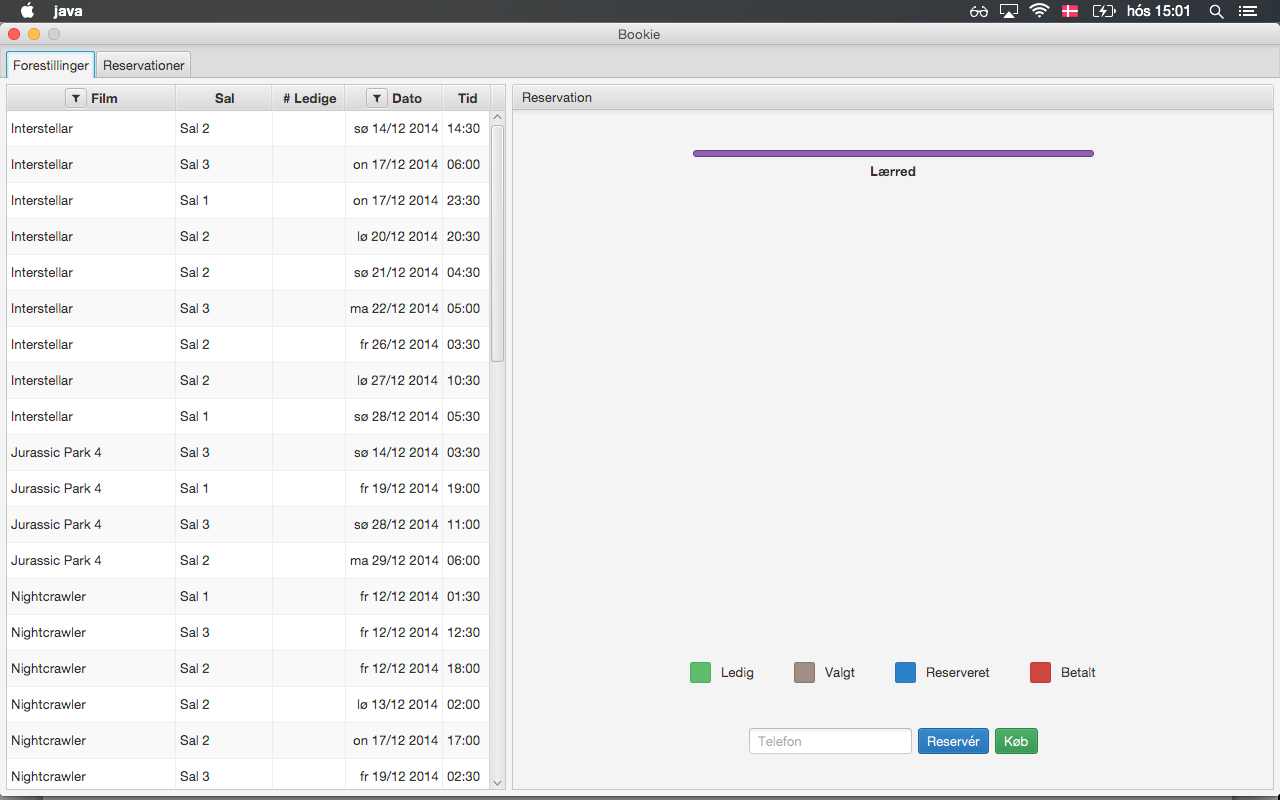
\includegraphics[width=0.4\textwidth]{OpenBookie.png}
  \caption{Bookie startside}
\end{figure}

Efter der er blevet valgt en forestilling, kan man se den tilhørende sal med tilhørende sæder. Disse sæder kan derefter vælges og trykkes på, hvilket resulterer i, at sæderne bliver grå i farven (dette kan også ses lige over telefonnummer-feltet). \textit{Figur 4.1}

\begin{figure} [h]
  \centering
  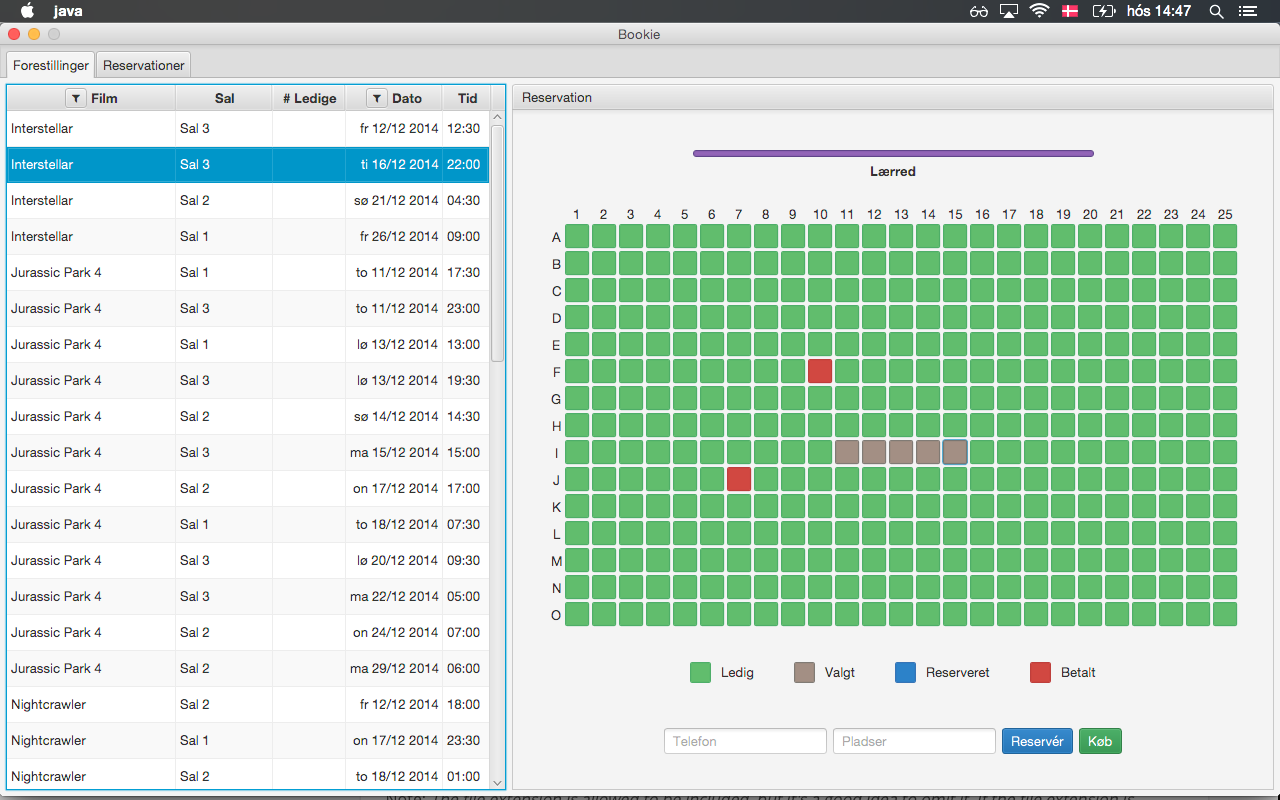
\includegraphics[width=0.4\textwidth]{ChosenSeats.png}
  \caption{Valgte sæder}
\end{figure}

Når telefonnummeret er blevet tastet ind og sæderne valgt, trykker man på \textit{Reservér} tasten, hvorefter sæderne bliver blå og viser ekspedienten, at reservationen er gennemført. Ses også i \textit{figur 4.3}

\begin{figure} [h]
  \centering
  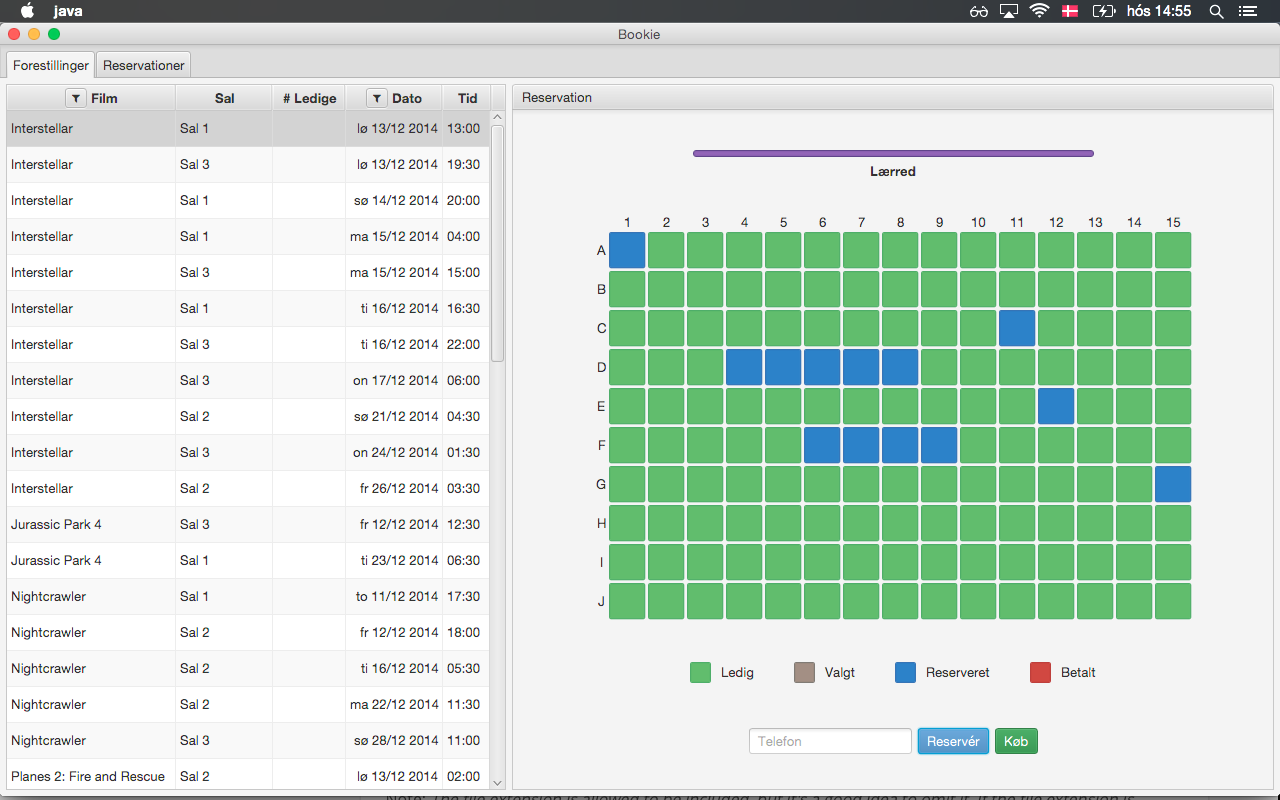
\includegraphics[width=0.4\textwidth]{ReserveredeSaeder.png}
  \caption{Reserverede Sæder}
\end{figure}

Efter at sæderne er reserverede, er det muligt at gå ind på \textit{Reservationer} oppe i venstre hjørne. Inde på denne side er det muligt at se alle eksisterende reservationer. 


